\setcounter{section}{99}
\section{Heavy-light decomposition. Тяжёлые и лёгкие рёбра. Лемма о числе лёгких рёбер на пути между двумя вершинами. Решение задачи обновления на ребре и суммы на пути за $O(log^2(n))$ на запрос.}

\textbf{Heavy-light decomposition}. Пулл задач: как на ДО, только в роли отрезков - пути в дереве. Числа написаны на каждом ребре.

Подвесим дерево за произвольную вершину r. Насчитаем размеры всех поддеревьев: subtree (см. предыдущие билеты на центроиды). Ребро из u в v - \textbf{тяжёлое}, если subtree[v] $\geqslant \frac{1}{2}$subtree[u]. Замечание: из каждой вершины выходит не более одного тяжёлого ребра. Вот эти тяжёлые рёбра можно склеить в пути; все остальные рёбра лёгкие.

Идея: разбили дерево на тяжёлые пути, между ними лёгкие рёбра. Тогда если мы хотим обновлять значение в ребре и находить сумму на пути между двумя вершинами, то мы хотим выстроить на тяжёлых путях деревья отрезков (котировать их как массивы, всё находить), а количество лёгких путей, которые надо будет доставить, будет немного.

\textbf{Лемма (о числе лёгких рёбер на пути между двумя вершинами)}. На пути от u до v ($\forall u, v$ количество лёгких рёбер равно $O(log(n))$).

$\blacktriangle$
Как устроен путь от u до v? Это путь от u до LCA и путь от LCA до v. Лёгкие рёбра, если мы проходим снизу вверх, увеличивают размер поддерева не менее, чем в два раза - в силу определения тяжёлого ребра, если бы это было неправдой, то мы только что прошли по тяжёлому ребру; отсюда на первом пути максимум логарифм лёгких рёбер; аналогичные рассуждения о пути вниз.
$\blacksquare$

Следствие: путь от u до v пересекает $O(log(n))$ тяжёлых путей.

Тогда обновление значения в ребре либо изменяет ДО на тяжёлом пути (если ребро тяжёлое), либо ребро лёгкое и ничего не меняется; первое делается за $O(log(n))$, второе - за $O(1)$.

Сумма ищется за $O(log(n)\cdot log(n) + 1\cdot log(n))$, где первое слагаемое - это из работы с тяжёлыми путями (тяжёлых путей логарифм, на каждом из них сумма ищется за логирифм), правая - работа с лёгкими путями (лёгких путей логарифм, работаем с ними за единицу). Тогда итоговая асимптотика - это лишь первое слагаемое, $O(log^2(n))$

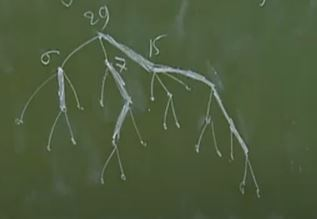
\includegraphics[]{images/100-102_heavy_light}

\setcounter{section}{100}
\section{Центроидная декомпозиция. Подсчёт числа объектов, обладающих заданным свойством.}

\textbf{Задача}: найти число объектов со свойством $\alpha$. Например, количество троек вершин, которые находятся на одном и том же расстоянии х друг от друга. Или количество путей, на которых сумма хорошая. Или на рёбрах написаны скобки, найти количество путей, образующих ПСП.

\textbf{Решение в общем виде}: Пусть С - центроид дерева Т.

1.Находим его за линейное время. Подвесим дерево за центроид, все размеры не больше половины исходного. Найдём количество объектов, для которых свойство $\alpha$ пропадёт, если удалить вершинку С. Как именно это сделать? Зависит от задачи.

2. Если $T_1, \dots, T_k$ - поддеревья, которые остались после удаления центроида - запускаемся рекурсивно от них (с удалённой вершинкой С). Таким образом, при запуске рекурсии мы минимум в два раза уменьшаем количество вершин в дереве на каждом шаге, значит, глубина рекурсии не превышает логарифм. Тогда если, например, пункт 1 реализован за $O(n)$, то суммарная сложность - $O(n log(n))$ 

Ответ - рекурсия, количество искомых свойств, на которых влияет удаление центроида плюс количество искомых свойств, на которых влияет удаление центроида из поддеревьев-детей предыдущего центроида и так далее. По сути мы просто разбили все искомые объекты так, чтобы их было проще считать.

\setcounter{section}{101}
\section{Центроидная декомпозиция. Задача о перекрашивании синих вершин в красный цвет и поиска расстояния до ближайшей красной вершины.}

\begin{figure}[!htb]
   \begin{minipage}{.5\textwidth}
     \centering
     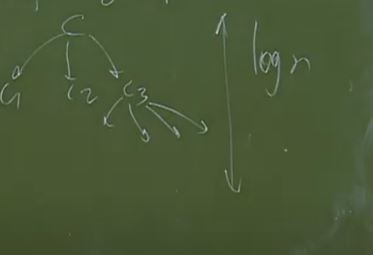
\includegraphics[height = 4 cm]{images/100-102_decomposition}
     \caption{Изображение дерева центроидов - 1.}
   \end{minipage}\hfill
    \begin{minipage}{.5\textwidth}
     \centering
     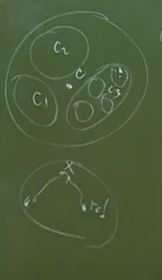
\includegraphics[height = 4 cm]{images/100-102_decomp2}
     \caption{Дерево центроидов 2 + поиск красной вершины.}
   \end{minipage}
\end{figure}

\textbf{Задача}. Дано дерево. Каждая вершина либо синяя, либо красная. Дано два типа запросов:

- перекрасить синюю v в красный цвет.

- для данной вершины u сообщить расстояние до ближайшей красной.

\textbf{Дерево центроидов} - корень дерева - исходный центроид, его дети - центроиды в поддеревьях, на которые мы разбились при рекурсии. Глубина дерева - максимум логарифм.


Запрос типа 2: искомая вершина лежит в одном из бОльших поддеревьев (наддеревьев). Она там лежит, так как по сути мы просто поднимаемся в более верхнее дерево, которое было до этого разбито на поддеревья, и когда-то поднимемся до всего дерева. Значит, в каком-то из наддеревьев лежит эта вершина.  Соотвественно, на произвольном шаге, где центроид х, хочется найти ближайшую к х красную вершину и сказать, что она же ближайшая к u, просто надо сначала дойти до х, потом до u. (см. рис. 2)

Доказательство: рассматриваем дерево, в котором лежат обе вершины (u и ближайшая к ней красная), а в следующих поддеревьях - не лежат, но тогда расстояние от u до красной - это расстояние до центроида + расстояние от центроида до красной.

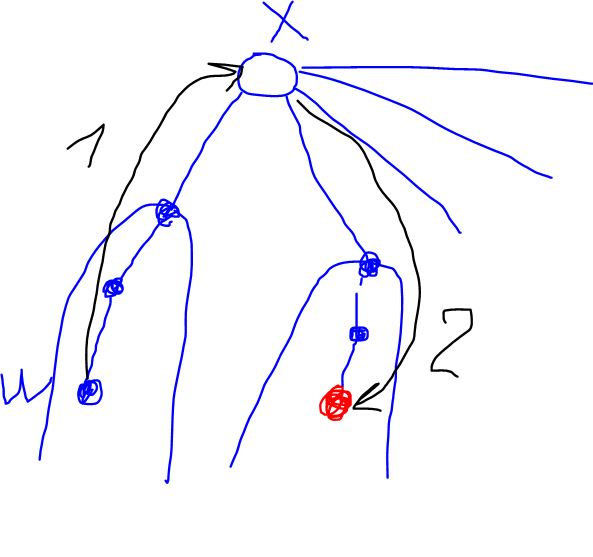
\includegraphics[height=4cm]{images/100-102_dist_red2}

Пусть $T_v$ - поддерево с центроидом v. Для каждой v находим ближайшую красную в $T_v$: closest[v] = $min_{r \in T_V} dist(v, r)$, где r - красная. Тогда ответ на запрос 2 типа - min по всем v - предки в деревне центроидов от $dist(u, v) + closest[v]$. Первое слагаемое вычисляется за логарифм (потому что мы умеем искать LCA за логарифм), значит, всё в итоге делается за $O(log^2(n))$.

Для запроса первого типа надо обновить closest для тех вершин v, для которых r стало лежать в $T_v$: в точности все предки вершины r. По всем v - предкам r в дереве центроидов берём новый closest - минимум из старого и нового. Время: $O(log^2(n))$, т.к. для каждого предка за логарифм обновляем расстояния до красной точки.